\documentclass[11pt]{article}
\usepackage[T1]{fontenc}
\usepackage{lmodern,microtype}
\usepackage[margin=0.9in]{geometry}
\usepackage{amsmath,amssymb,mathtools,bm,booktabs,array,graphicx,xcolor}
\usepackage[colorlinks=true,linkcolor=blue!45!black,urlcolor=blue!55!black,citecolor=blue!45!black]{hyperref}
\hypersetup{pdftitle={Local Type 0B conformal blocks and correlator assembly},
 pdfauthor={Machine note},pdfsubject={Sphere four-point and torus two-point production conventions}}
\usepackage{fancyhdr}
\usepackage{placeins}
\pagestyle{fancy}
\fancyhf{}\fancyhead[L]{Local Type 0B conformal blocks}\fancyhead[R]{Production convention}
\fancyfoot[C]{\thepage}
\setlength{\headheight}{14pt}
\setlength{\emergencystretch}{2em}
\newcommand{\NS}{\mathrm{NS}}
\newcommand{\R}{\mathrm{R}}
\newcommand{\U}{\Upsilon}
\newcommand{\Ct}{\widetilde C}
\newcommand{\F}{\mathcal F}
\newcommand{\dd}{\mathrm d}
\newcommand{\code}[1]{\texttt{\small #1}}
\newcommand{\barF}{\overline{\mathcal F}}
\DeclareMathOperator{\Tr}{Tr}
\title{\textbf{Super-Liouville conformal blocks}\\
  \large Sphere four-point and torus two-point decompositions\\
  in the local Type 0B amplitude convention}
\author{Machine note accompanying the standalone source package}
\date{Local source snapshot: 24 September 2026}
\begin{document}
\maketitle
\begin{abstract}
This note specifies the coefficients, nonchiral contractions and numerical
block algorithms used by the local amplitude code. It covers four NS,
two NS and two R, and four R external fields on the sphere, and NS or R
external fields on the torus. The three-point constants are explicit.
The sphere scattering half-sum Ramond dictionary is retained; its
conversion to the separate equal-metric sewing convention is described,
rather than silently applied. Fresh coefficient and sphere crossing
checks accompany the package. The Type 0B sphere amplitude plot uses
retained production data. The RR torus has a fixed relative correlator
normalization, but its common string-amplitude constant and integrated
amplitude remain undetermined.
\end{abstract}
\tableofcontents

\section{Conventions and scope}
The authority for the formulas below is the local source snapshot,
including local convention repairs, with base commit
\code{488710430}. Copied scientific files are unchanged, and their hashes
are recorded in \code{provenance/source\_origins.json}.
The earlier machine notes are retained in \code{notes/originals}.
We use
\begin{equation}
 b=1,\quad Q=2,\quad c=\frac32+3Q^2=\frac{27}{2},\qquad
 h_\NS(P)=\frac{1+P^2}{2},\quad h_\R(P)=\frac9{16}+\frac{P^2}{2}.
 \label{eq:weights}
\end{equation}
The ordinary central charge \(c\), not \(\hat c=2c/3\), enters the
recursions. Internal continuum momenta are positive. External momenta
are analytically continued when necessary. A bar on a block denotes
the specified antichiral frame at the same physical momenta; at
complex momentum it is not generally complex conjugation of the
whole numerical block.

\begin{center}
\begin{tabular}{p{.21\linewidth}p{.35\linewidth}p{.33\linewidth}}
\toprule
Quantity & Block evaluation & Nonchiral convention\\ \midrule
NS sphere & Multiprecision NS \(c\)-recursion and elliptic re-expansion &
BRY \(G,H,J\), with one odd-block sign conversion\\
R-containing sphere & Two Virasoro recursions, finite branching,
assembled self-dual limit & Graded component sum, analytic dual,
scattering half-sum fields\\
NS torus punctures & NS necklace \(c\)-recursion and conditioned R
Ward/Gram contraction & Stored form phases and \(E/2,O/2\)\\
R torus punctures & NS/R radial trace and RR-pair OPE with handle traces &
Original state sums followed by relative correlator prefactors\\
\bottomrule
\end{tabular}
\end{center}

\section{Explicit production three-point coefficients}
\label{sec:constants}
Let \(G_B\) be the Barnes \(G\)-function. The exact \(b=1\) functions
in the production structure-constant module are
\begin{align}
 \U_1(x)&=G_B(x)G_B(2-x),\qquad \U_1(1)=1,\\
 \U_\NS(x)&=\U_1(x/2)\U_1(1+x/2)\nonumber\\
 &=\Gamma(x/2)\Gamma(1-x/2)G_B(x/2)^2G_B(1-x/2)^2,\\
 \U_\R(x)&=\U_1((x+1)/2)^2.
\end{align}
The code uses the second expression for \(\U_\NS\), setting
\(\U_\NS(0)=0\) explicitly. Define
\begin{equation}
 N_\NS(P)=\frac{\Gamma(1+iP)}{\Gamma(1-iP)}\U_\NS(2iP),\qquad
 N_\R(P)=\frac{\Gamma(\frac12+iP)}{\Gamma(\frac12-iP)}\U_\R(2iP).
 \label{eq:legs}
\end{equation}
For three momenta write
\[
 S=P_1+P_2+P_3,\quad
 D_1=P_2+P_3-P_1,\quad D_2=P_1+P_3-P_2,\quad D_3=P_1+P_2-P_3.
\]
The actual NS functions are
\begin{align}
 C(P_1,P_2,P_3)&=\frac{i}{2}
 \frac{\prod_jN_\NS(P_j)}
 {\U_\NS(1+iS)\prod_j\U_\NS(1+iD_j)},\label{eq:C}\\
 \Ct(P_1,P_2,P_3)&=i
 \frac{\prod_jN_\NS(P_j)}
 {\U_\R(1+iS)\prod_j\U_\R(1+iD_j)}.\label{eq:Ct}
\end{align}
They are real for positive real momenta in the BRY phase convention
\cite{BRY}. The displayed \(i\)'s are part of the analytic definitions.
For \(R(P_1)R(P_2)V(P_3)\), the two raw returned functions are
\begin{align}
 E(P_1,P_2;P_3)&=-\frac{i}{2}
 \frac{N_\R(P_1)N_\R(P_2)N_\NS(P_3)}
 {\U_\R(1+iS)\U_\R(1+iD_3)\U_\NS(1+iD_1)\U_\NS(1+iD_2)},
 \label{eq:E}\\
 O(P_1,P_2;P_3)&=-\frac{i}{2}
 \frac{N_\R(P_1)N_\R(P_2)N_\NS(P_3)}
 {\U_\NS(1+iS)\U_\NS(1+iD_3)\U_\R(1+iD_1)\U_\R(1+iD_2)}.
 \label{eq:O}
\end{align}
The first two arguments are Ramond and the third is NS.

\subsection{Halves, phases and the factors of two and four}
The sphere scattering fields and local torus trinion adapters use
\begin{equation}
 c_+=E/2,\qquad c_-=O/2,\qquad
 d_\epsilon=c_++\epsilon c_-=(E+\epsilon O)/2.
 \label{eq:sc-dictionary}
\end{equation}
Here \(c_\eta\) labels an HJS sign form; \(d_\epsilon\) labels a
physical Ramond-family ground three-point amplitude. The NS graded
sewing coefficients are
\begin{equation}
 \Gamma_0=C,\qquad \Gamma_1=i\Ct,\qquad
 -\Gamma_{L,1}\Gamma_{R,1}=+\Ct_L\Ct_R.
 \label{eq:ns-phase}
\end{equation}
The same \(i\) occurs at both vertices in a bilinear coefficient product;
using an absolute square would lose this sign.

The independent sphere sewing-metric audit finds that the half-sum
scattering field has effective
\begin{equation}
 D_{\R,\mathrm{sc}}=\tfrac12D_\NS,\qquad
 D_\NS(P,P')=\pi\delta(P-P').
 \label{eq:metric}
\end{equation}
For an NS identity insertion \(P_3=i(1-\varepsilon)\),
\((E+O)/(2C)\to1/2\). The R-exchange density absorbs the relative
inverse metric: a printed common \(\dd P/\pi\) alone does not determine
the metric. The finite reduced R ground vector still has unit norm.

The other machine note's equal-metric dictionary is
\(\widehat c=(E,O)\). A consistent conversion is
\begin{equation}
 \widehat R=\sqrt2R_{\mathrm{sc}},\qquad
 \widehat D_\R=2D_{\R,\mathrm{sc}},\qquad
 \widehat d_\epsilon=2d_\epsilon.
\end{equation}
It multiplies a mixed Liouville correlator by two and a four-R
Liouville correlator by four. The coefficients of the same physical
axion vertex then contribute \(1/\sqrt2\) per R leg, canceling this
change in the amplitude. Doubling two vertices with all other data
fixed instead multiplies their contribution by four.
No extra multiplier of this kind is applied here.
The later RR torus factors in Section~\ref{sec:rr-torus} are an
overall correlator normalization and do not change state metrics.

\section{Sphere four-point decompositions}
Momenta \((P_1,P_2,P_3,P_4)\) are assigned to \((0,z,1,\infty)\).
Evaluated blocks include coordinate powers, but exclude structure
constants and spectral measures.

\subsection{Four NS external states}
Let \(P_e,P_o\) be the BRY-facing bottom-field blocks and
\(D_e,D_o\) the blocks with \(G_{-1/2}\) on legs 2 and 3.
In terms of the stored fixed-parity blocks,
\[
 P_e=F_e,\quad P_o=-F_o,\qquad
 D_e=F_e^{**},\quad D_o=-F_o^{**}.
\]
The stored unstarred odd block begins
\(F_o=-z^{h-h_1-h_2+1/2}/(2h)+\cdots\).
Put \(C_L=C(P_4,P_3,P)\), \(C_R=C(P,P_2,P_1)\), and similarly
for \(\Ct\). The implemented decomposition is
\begin{align}
 G&=\int_0^\infty\frac{\dd P}{\pi}
 [C_LC_RP_e\bar P_e+\Ct_L\Ct_RP_o\bar P_o],\label{eq:G}\\
 H&=-\int_0^\infty\frac{\dd P}{\pi}
 [\Ct_L\Ct_RD_e\bar D_e+C_LC_RD_o\bar D_o],\\
 J&=-\int_0^\infty\frac{\dd P}{\pi}
 \left[C_LC_R\left(\frac{D_o\bar P_e}{1-\bar z}
                         +\frac{P_e\bar D_o}{1-z}\right)
 +\Ct_L\Ct_R\left(\frac{D_e\bar P_o}{1-\bar z}
                         +\frac{P_o\bar D_e}{1-z}\right)\right].
\end{align}
The antichiral functions evaluate the same analytic coefficient table
at \(\bar z\). \(H,J\) include the specific descendant and free-fermion
combinations of BRY Appendix A; they are not arbitrary scalar
four-point functions.

\subsection{R external fields: explicit component sum}
The stored families and ordered external sectors are
\[
\begin{array}{c|c|c}
 \text{family}&(s_1,s_2,s_3,s_4)&\text{internal sector}\\ \hline
 \texttt{mixed\_ns}&(\R,\R,\NS,\NS)&\NS\\
 \texttt{mixed\_r}&(\NS,\R,\R,\NS)&\R\\
 \texttt{rrrr}&(\R,\R,\R,\R)&\NS .
\end{array}
\]
An NS component is the pair \((a,\bar a)\) in
\(G_{-1/2}^{a}\bar G_{-1/2}^{\bar a}V\), in that fixed order.
An R family \(e=0,1\) has coefficients
\begin{equation}
 u_0=\frac1{\sqrt2}(1,0,0,-i)^T,\qquad
 u_1=\frac1{\sqrt2}(0,1,1,0)^T
 \label{eq:Rstates}
\end{equation}
in the ground basis \((++,+-,-+,--)\).
For an NS endpoint \(u\) is instead the delta function selecting its
component bits. Middle R fields have chiral block bit zero; their
physical family enters
\begin{equation}
 V_e^\eta(r,\bar r)=\delta_{r+\bar r,e\ {\rm mod}\,2}\frac1{\sqrt2}
 \begin{cases}(-i)^r,&e=0,\\ \eta,&e=1.\end{cases}
 \label{eq:Rvertex}
\end{equation}

The stripped spectral weights have no implicit fitted constant.
Write \(\alpha_j=1+iP_j,\ \alpha_\pm=1\pm iP\), and define
\begin{align}
 {\cal D}_t(a,b,c)&=\U_{S_t}(a+b+c-2)
 \U_{S_t}(a+b-c)\U_{S_t}(a+c-b)\U_{S_t}(b+c-a),
 \quad S_0=\NS,\ S_1=\R,\\
 {\cal R}_\eta(n;r,s)&=\U_{A_\eta}(n+r+s-2)\U_{A_\eta}(r+s-n)
 \U_{B_\eta}(n+r-s)\U_{B_\eta}(n+s-r),\\
 (A_+,B_+)&=(\R,\NS),\qquad(A_-,B_-)=(\NS,\R),\qquad
 W_S(P)=\U_S(2\alpha_+)\U_S(2\alpha_-).
\end{align}
The densities used by the code are
\begin{align}
 \rho_{\rm mixed\_ns}(t;1,\eta_R)
 &=\frac{2^tW_\NS(P)}
 {{\cal D}_t(\alpha_4,\alpha_3,\alpha_+)
  {\cal R}_{\eta_R}(\alpha_-;\alpha_2,\alpha_1)},\\
 \rho_{\rm mixed\_r}(0;\eta_L,\eta_R)
 &=\frac{W_\R(P)}
 {{\cal R}_{\eta_L}(\alpha_4;\alpha_3,\alpha_+)
  {\cal R}_{\eta_R}(\alpha_1;\alpha_2,\alpha_-)},\\
 \rho_{\rm rrrr}(0;\eta_L,\eta_R)
 &=\frac{W_\NS(P)}
 {{\cal R}_{\eta_L}(\alpha_+;\alpha_3,\alpha_4)
  {\cal R}_{\eta_R}(\alpha_-;\alpha_2,\alpha_1)}.
 \label{eq:r-densities}
\end{align}
The external factor restoring these stripped densities is
\begin{equation}
 {\cal N}=\frac{(-1)^{n_R/2}}{2^{2+n_R/2}}
                   \prod_{j=1}^4N_{s_j}(P_j)
 =\begin{cases}-\frac18\prod_jN_{s_j}(P_j),&n_R=2,\\
                \frac1{16}\prod_jN_\R(P_j),&n_R=4.\end{cases}
 \label{eq:external-N}
\end{equation}

Sum independently over \(k,\bar k=0,1\), the endpoint components
\((a_1,\bar a_1),(a_4,\bar a_4)\), and \(\eta_L,\eta_R=\pm1\).
Set \(a_2=\bar a_2=0\). On leg 3 use its NS bits, or zero for R.
All following bit equations are modulo two:
\[
 r=k+a_1,\quad\bar r=\bar k+\bar a_1,\qquad
 l=a_4+k,\quad\bar l=\bar a_4+\bar k.
\]
For mixed NS, restrict \(\eta_L=1\), set
\(t=l+a_3,\ \bar t=\bar l+\bar a_3\), and take
\[
 {\cal L}=\delta_{t,\bar t}(-1)^{t(1+\bar a_3)}i^t,\qquad
 \rho=\rho_{\rm mixed\_ns}(t;1,\eta_R).
\]
For the other families take
\({\cal L}=V_{e_3}^{\eta_L}(l,\bar l)\) and their \(t=0\) density.
Let \(\chi_R=1\) only for internal R, and
\(\eta_R'=(-1)^{\chi_R}\eta_R\). The full correlator is
\begin{align}
 {\cal G}_{\bm e}(z,\bar z)
 &=\int_0^\infty\frac{\dd P}{\pi}{\cal N}
 \sum u_{e_1}(a_1,\bar a_1)u_{e_4}(a_4,\bar a_4)^*
 (-1)^{\bar r a_1+\bar l k+\chi_R(r+\bar r)}
 {\cal L}V_{e_2}^{\eta_R}(r,\bar r)\rho\nonumber\\
 &\hspace{28mm}\times
 \F_k^{\eta_L,\eta_R'}(z;\bm a)
 \barF_{\bar k}^{\eta_L,\eta_R'}(\bar z;\bar{\bm a}).
 \label{eq:fullR}
\end{align}
The star on \(u_{e_4}\) conjugates its fixed phase, not \(P_4\).
Both the internal-R sign reflection and the extra parity factor are
essential. The production does not replace this sum by a guessed
\(\sum|\F|^2\). For complex momenta it constructs a dual table at
\((\bm P^*,P^*)\), then conjugates its value:
\(\barF(\bar z;\bm P)=[\F(z;\bm P^*)]^*\).
The native sign and small-representation conventions are those of
the corrected Ramond formulas in \cite{Suchanek,HJS}.

\section{How the sphere blocks are evaluated}
\subsection{Definition and NS coefficient recursion}
The local SCA has
\begin{align}
 [L_m,L_n]&=(m-n)L_{m+n}+\frac c{12}(m^3-m)\delta_{m+n,0},\\
 [L_m,G_r]&=(m/2-r)G_{m+r},\quad
 \{G_r,G_s\}=2L_{r+s}+\frac c3(r^2-\tfrac14)\delta_{r+s,0}.
\end{align}
PBW bases put ordered negative \(L\) modes before distinct ordered
negative \(G\) modes, reducing \(G_{-r}^2=L_{-2r}\).
R zero modes act on the ground doublet. At level \(\ell\) the
definition is the ordered Ward contraction
\begin{equation}
 f_\ell=\sum_{|I|=|J|=\ell}
 \rho_L(v_4,v_3,I)(B_\ell^{-1})^{IJ}\rho_R(J,v_2,v_1).
 \label{eq:gram}
\end{equation}
Ground-frame factors belong to \(\rho\) and \(B\), once.
The NS seeds are \(\rho_0(\nu,\nu,\nu)=1\) and
\(\rho_1(\nu,G_{-1/2}\nu,\nu)=1\).

The NS code uses a memoized \(c\)-recursion to compute
\eqref{eq:gram}. Write \(F_N=f_{N/2}\), let \(s_2,s_3\) be the
external star bits, and set \(A=h+h_3-h_4,\ B=h+h_2-h_1\).
Its large-\(c\) seeds are
\begin{align}
 f_{2m}^{(\infty)}
 &=\frac{(A+s_3/2)_m(B+s_2/2)_m}{m!(2h)_m},\\
 f_{2m+1}^{(\infty)}
 &=-\frac{X_{s_3}(A,m)X_{s_2}(B,m)}{m!(2h)_{m+1}},
 \quad X_0(x,m)=(x+\tfrac12)_m,\quad X_1(x,m)=(x)_{m+1}.
\end{align}
For \(r\ge2,s\ge1,r+s\) even, define
\begin{align}
 \Delta&=\sqrt{16h^2+8(rs-1)h+(r-s)^2},&
 x_{rs}&=-\frac{4h+rs-1+\Delta}{r^2-1},\\
 b_{rs}&=\sqrt{x_{rs}},&
 c_{rs}&=\frac{15}{2}+3x_{rs}+3/x_{rs},\quad
 J_{rs}=-\partial_hc_{rs}.
\end{align}
The code chooses the sign of \(\Delta\) giving the larger-magnitude
numerator, the standard continuation of positive real \(h\). Let
\begin{align}
 A_{rs}(b)&=\frac12
 \prod_{\substack{p=1-r,\ldots,r;\ q=1-s,\ldots,s\\p+q\ {\rm even}\\
                  (p,q)\ne(0,0),(r,s)}}\frac{\sqrt2}{pb+q/b},\\
 {\cal P}_{rs}^a(h_i,h_j;b)&=
 \prod_{\substack{p=1-r,\,3-r,\ldots,r-1\\q=1-s,\,3-s,\ldots,s-1\\
                  p+q-r-s\equiv2(1-a)\;({\rm mod}\ 4)}}
 \frac{(\lambda_i-\lambda_j+pb+q/b)(\lambda_i+\lambda_j+pb+q/b)}8,\nonumber\\
 &\hspace{15mm}\lambda_j=\sqrt{(b+b^{-1})^2-8h_j}.
\end{align}
Then
\begin{align}
 F_N(h,c)&=f_N^{(\infty)}(h)+\sum_{\substack{r\ge2,s\ge1,\ r+s\ {\rm even}\\rs\le N}}
 \frac{R_{rs}^{(N)}(h)}{c-c_{rs}(h)}
 F_{N-rs}(h+rs/2,c_{rs}),\label{eq:ns-recursion}\\
 R_{rs}^{(N)}(h)&=(-1)^{rs}J_{rs}A_{rs}
 {\cal P}_{rs}^{s_2\oplus(N\bmod2)}(h_1,h_2)
 {\cal P}_{rs}^{s_3\oplus(N\bmod2)}(h_4,h_3).\nonumber
\end{align}
The endpoint \(rs=N\) is included. Each call lowers \(N\);
the supplied sphere examples use 60-digit coefficient arithmetic.

The local block is
\(z^{h-h_1-h_2-s_2/2}\sum_NF_Nz^{N/2}\) with one parity retained.
Put \(q=e^{i\pi\tau_z}\), \(\tau_z=iK(1-z)/K(z)\) and
\(d_j=h_j+s_j/2\), with \(s_1=s_4=0\). Its elliptic prefactor is
\begin{equation}
 (16q)^{h-Q^2/8}z^{Q^2/8-d_1-d_2}(1-z)^{Q^2/8-d_2-d_3}
 \theta_3(q)^{3Q^2/2-4\sum_jd_j}.
\end{equation}
The remaining coefficients are obtained by the formal substitution
\(z=\theta_2(q)^4/\theta_3(q)^4\) and division by this prefactor.
No new fitted elliptic seed is inserted. The ordinary \code{order}
counts coefficients in each parity. BRY order \(L\) instead retains
even powers through \(q^L\) and odd powers through \(q^{L-1/2}\).

\subsection{R blocks: branching, auxiliary division and self-dual limit}
The production tensors the SCA with an auxiliary Majorana module and
decomposes it into two commuting Virasoro modules at generic \(b\).
The correlated roots are
\begin{equation}
 b_1=\sqrt{\frac{2b^2}{1-b^2}},\quad b_2^{-1}=\sqrt{\frac2{b^2-1}},
 \quad d_1=\sqrt{2-2b^2},\quad d_2=-b_2^{-1}d_1/b_1.
\end{equation}
For sphere momentum \(P\), the branch \(n\) has
\begin{align}
 p_n^{(1)}&=-iP/d_1+nb_1,\qquad p_n^{(2)}=-iP/d_2+n/b_2,\\
 c_j&=1+6(b_j+b_j^{-1})^2,\qquad
 h_n^{(j)}=\tfrac14(b_j+b_j^{-1})^2-(p_n^{(j)})^2.
\end{align}
The sign \(-iP\) implements the sphere frame \(\beta=-iP/\sqrt2\).
The marked torus Ward source has its separately fixed
\(\beta=+iP/\sqrt2\), and its tensors are not silently substituted here.

The finite tensor PBW basis at the branch grade is constructed.
The known \(L_0^{(1)}\) eigenvalue \(h_n^{(1)}\) gives a constrained
linear solve for the highest vector \(v_n\), with bilinear norm
\(v_n^TBv_n\). Diagonal balancing, isolation tests and high-precision
residual checks precede the branch sum; assembly retains 60 digits.
An external state is resolved by a finite linear solve in branch
vectors, with labels \(0\) for an NS bottom state, \(\pm1/2\) for
its \(G_{-1/2}\) component, and \(\pm1/4\) for an R ground.

In the linear sign frame the finite enlarged descendant block is
\begin{equation}
 \F_{\rm enl}(z)=\sum_{n,\bm\nu}
 \frac{\prod_jt_{j,\nu_j}\,
 \rho_L(v_{\nu_4},v_{\nu_3},v_n)
 \rho_R(v_n,v_{\nu_2},v_{\nu_1})}{\langle v_n,v_n\rangle}
 z^{g_n}{\cal V}_1(z){\cal V}_2(z).
 \label{eq:branch-sum}
\end{equation}
Here \(t\) are external resolution coefficients,
\(g_n=2n^2\) in NS and \(g_n=2n^2-1/8\) in R.
Only \(2g_n\le N\) is kept; NS also requires \(2n\bmod2=k\).
Each \({\cal V}_j\) is the unit-leading ordinary Virasoro block at
the displayed branch weights, computed by sphere \(c\)-recursion;
their series are convolved through the remaining order.
Explicitly, its coefficients are
\begin{align}
 v_m(c,h)&=\frac{(h+h_2-h_1)_m(h+h_3-h_4)_m}{m!(2h)_m}\nonumber\\
 &\quad+\sum_{\substack{r\ge2,s\ge1\\rs\le m}}
 \frac{J^{\rm V}_{rs}A^{\rm V}_{rs}
 P^{\rm V}_{rs}(h_4,h_3)P^{\rm V}_{rs}(h_1,h_2)}{c-c^{\rm V}_{rs}}
 v_{m-rs}(c^{\rm V}_{rs},h+rs),\\
 x^{\rm V}_{rs}&=
 \frac{rs-1+2h+\sqrt{(r-s)^2+4(rs-1)h+4h^2}}{1-r^2},\qquad
 c^{\rm V}_{rs}=13+6(x^{\rm V}_{rs}+1/x^{\rm V}_{rs}),\\
 J^{\rm V}_{rs}&=-\partial_h c^{\rm V}_{rs},\qquad
 A^{\rm V}_{rs}=\frac12
 \prod_{\substack{p=1-r,\ldots,r;\ q=1-s,\ldots,s\\
 (p,q)\ne(0,0),(r,s)}}(pb+q/b)^{-1},\\
 P^{\rm V}_{rs}(h_i,h_j)&=
 \prod_{\substack{p=1-r,3-r,\ldots,r-1\\q=1-s,3-s,\ldots,s-1}}
 \frac{(\lambda_i+\lambda_j+pb+q/b)(\lambda_i-\lambda_j+pb+q/b)}4.
\end{align}
Here \(b=\sqrt{x^{\rm V}_{rs}}\) and
\(\lambda_j=\sqrt{(b+b^{-1})^2-4h_j}\) only within the Virasoro
residue. If the displayed root is numerically zero, the code uses
the other finite root. It algebraically cancels common factors in
\(J^{\rm V}A^{\rm V}\) before numerical evaluation; unresolved poles
raise an error. This recurrence is evaluated at 60 digits in the
production precision bootstrap.
The ordinary Virasoro recurrence follows the sphere specialization
of \cite{CCY}; the finite branching and frame conversion are specified
by the preserved local sources.

Branch vertices are evaluated by expanding the finite vectors and
applying the ordered physical and auxiliary Ward forms with their
graded tensor signs. No unverified closed Ramond branching product
is used as the definition.

Remove the external polynomial-ground scales and divide the formal
series, coefficient by coefficient, by the unit-leading auxiliary block
\begin{equation}
 A_{\rm mixed\_ns}=1,\qquad
 A_{\rm mixed\_r}=(1-z)^{-1/8},\qquad
 A_{\rm rrrr}=(1-z)^{-1/8}\sqrt{\frac{1+\sqrt{1-z}}2}.
\end{equation}
Their leading \(z\) powers are already stripped. Define
\[
 T=\tfrac12\begin{pmatrix}1-i&1+i\\1+i&1-i\end{pmatrix},\qquad
 T_f=\operatorname{diag}(1,(-1)^f)T.
\]
The native sign vector is \(M^{-1}\F_{\rm linear}\), with \(M=I\)
for mixed NS, \(I_2\otimes T_{k+a_2+a_1}\) for mixed R, and
\(i^{a_4}T_{a_4+a_3+k}\otimes I_2\) for four R, in sign order \(+,-\).

At fixed momenta and component labels, the \emph{assembled native
coefficient} is extrapolated as
\begin{equation}
 f(1)\simeq
 \frac{4(1+\epsilon)f(1+\epsilon)-(1+2\epsilon)f(1+2\epsilon)}
 {3+2\epsilon},\qquad \epsilon=0.01.
 \label{eq:extrapolation}
\end{equation}
This cancels the leading dependence on \(Q-2=(b-1)^2/b\).
Formal \(O(\epsilon^4)\) accuracy assumes analyticity and \(b\)-duality;
it is not a certified error estimate. Singular individual Virasoro
factors are not extrapolated separately.

Finally use the exact \(b=1\) prefactors. For
\(d_j=h_{s_j}(P_j)+a_j/2\) on NS legs and \(d_j=h_\R(P_j)\) on R,
and \(B_0=Q^2/8=1/2\),
\begin{align}
 \F(z)&=(16q)^{P^2/2}z^A(1-z)^B\theta_3(q)^K
                         \sum_{j=0}^{N}h_jt^j,\qquad t=e^{i\pi\tau_z/2},\\
 A&=B_0-d_1-d_2+\tfrac1{16}{\bf1}_{\rm mixed\_r},\\
 B&=B_0-d_2-d_3+\tfrac1{16}{\bf1}_{\rm mixed\_ns},\qquad
 K=12B_0-4\sum_jd_j+\tfrac12{\bf1}_{\rm not\ rrrr}.
\end{align}
The \(h_j\) follow by finite formal substitution of the calculated
\(z\)-coefficients. The half-nome is taken from \(\tau_z\), not an
independently chosen square root. Cuts need a consistent marked lift.

\section{Torus two-point decompositions}
\subsection{NS external fields: production necklace}
The punctures are \(0,z\), with periods \(1,\tau\), and
\begin{equation}
 \log q_0=2\pi iz,\qquad \log q_1=2\pi i(\tau-z),\qquad
 0<\operatorname{Im}z<\operatorname{Im}\tau.
\end{equation}
Keep these unwrapped logs. Both external Liouville momenta are
\(\omega\); internal \(P_0,P_1\) are independent. For homogeneous
forms \(f=(f_0,f_1)\) and external word \(w\), the descendant series is
\begin{equation}
 F_{w,f}=\sum_{\ell_0,\ell_1}q_0^{\ell_0}q_1^{\ell_1}
 \sum\rho_{f_0}(I_1,w_0,J_0)(B_0^{-1})^{J_0I_0}
     \rho_{f_1}(I_0,w_1,J_1)(B_1^{-1})^{J_1I_1}.
 \label{eq:necklace}
\end{equation}
The source vertex contains its ordered phases. In NS, \(N_j=2\ell_j\)
and \(N_{v-1}+N_v+w_v=f_v\pmod2\), with \(w_v=0,1\) for bottom
and \(G_{-1/2}\) fields.

The NS graph recursion sums over a Kac pole on either edge, subtracts
\(rs\) from that edge's twice-level, shifts its weight by \(rs/2\),
and flips both incident form bits if \(rs\) is odd.
The kernel is \((-1)^{rs}JA{\cal P}_L{\cal P}_R\), using the functions
in \eqref{eq:ns-recursion}; for edge \(e\) the endpoint weight pairs are
\((h_{e+1},d_{e+1})\) and \((h_{e-1},d_e)\), cyclically.
The regular term is the global \(osp(1|2)\) necklace convolved with
the non-global vacuum modes, which shift both edge levels equally.
Explicitly, with \(\mathfrak q=q_0q_1\) and
\(\sigma=(-1)^{f_0+f_1}\), that vacuum factor is
\[
 \chi_{\rm ng}(\mathfrak q)=\prod_{n=2}^{\infty}
 \frac{1+\sigma\mathfrak q^{n-1/2}}{1-\mathfrak q^n}
 =\sum_{K\ge0}\chi_K\mathfrak q^{K/2},\qquad
 f^{(\infty)}_{N_0,N_1}=\sum_{K=0}^{\min(N_0,N_1)}
 \chi_K f^{\rm global}_{N_0-K,N_1-K}.
\]
Global states \(L_{-1}^nG_{-1/2}^{\epsilon}|h\rangle\) have norm
\(n!(2h)_{n+\epsilon}\). Their forms follow from the finite global
Ward identities. The adapter multiplies the final coefficient by
\((-1)^{\sum_vf_vN_v}\) to obtain the production component tensor.
At total twice-level 15 and above, preparation tests successive
60--120 digit evaluations to scaled tolerance \(10^{-11}\).
Guarded confluent cases use the source's checked contour average.

R internal edges use a direct conditioned PBW calculation instead.
At each level both ground parities are kept, Gram matrices are split
by full state parity, diagonally equilibrated and Cholesky factored.
Whitening each vertex and taking the finite matrix trace evaluates
\eqref{eq:necklace} without explicitly forming a poorly conditioned
inverse. External NS-weight dependence is evaluated as a finite
polynomial at the actual complex energy.
An R supertrace inserts full state parity, including its ground
parity; integer descendant level is not that parity.
The cutoff is total twice-level \(N_0+N_1\le N_{\max}\).

The adapter returns GG/GG, GG/PP, PP/GG and PP/PP cylinder components.
Let \(H_G=-(-1)^fF_G,\ H_P=F_P\), with \(f=f_0=f_1\).
The PP pairing phase is one for NS internal states and \((-1)^f\)
for R internal states. The fixed-momentum
components are
\begin{equation}
 {\cal L}^{ab}_\delta=
 \frac1{\pi^2}\prod_{j=0}^1
 e^{(h_s(P_j)-c/24)(\log q_j+\overline{\log q_j})}
 \sum_{\lambda}K_\lambda H_{a,\lambda}\bar H_{b,\lambda},
 \qquad a,b=G,P,
 \label{eq:torus-components}
\end{equation}
where
\begin{align}
 K_f^\NS&=\prod_{v=0}^1C_{f_v}(P_{v-1},\omega,P_v),
                    &&(C_0,C_1)=(C,\Ct),\\
 K_{f,\eta_0,\eta_1}^{\R}
 &=(-1)^f\prod_{v=0}^1\left[\frac{B_{\eta_v}(P_{v-1},P_v;\omega)}2\right],
                    &&(B_+,B_-)=(E,O).
\end{align}
In particular, two Ramond trinions supply \(1/4\), with the odd
pairing sign retained. More generally, the code's ordered pairing
phase for external words \(a,b\) is
\[
 \Phi_s(f;a,b)=(-i)^{\sum b_v+\mathbf1_{s=\NS}\sum f_v}
 (-1)^{\sum f_vb_v+\sum_{i<j}(f_i+b_i)(f_j+a_j)}.
\]
The component adapter uses the PP weights \(a=b=(0,0)\), after
converting the GG chiral series as above.
NS supertrace supplies \((-1)^{N_1}\) in each chiral series.
R supertrace uses the state-parity insertion described above.
The antichiral table keeps the same analytic coefficients and
conjugates the geometric powers.
External \(2\pi\) coordinate factors, the GG factors \(\pm2\pi i\)
in the PCO terms, and time/ghost factors are outside
\eqref{eq:torus-components}. The adapter states that convention.
Its R supertrace is a Liouville component, not a completed odd-spin
string density.

\subsection{R external fields: radial and OPE channels}
\label{sec:rr-torus}
An R puncture changes the propagating sector. The radial sum has
one NS and one R edge, with times
\[
 (t_\NS,t_\R)=
 \begin{cases}(z,\tau-z),&\delta=1,2,\\
              (\tau-z,z),&\delta=3,4,\end{cases}
\]
where \(\delta\) labels \(\theta_1,\theta_2,\theta_3,\theta_4\).
Let \(A^{e,\delta}_{n,\bar n,r,\bar r}\) be the two full physical
NSRR vertices contracted with inverse NS and reduced-R Grams at
levels \((n/2,\bar n/2;r,\bar r)\), computed by the numeric NRR Ward
engine with \eqref{eq:Rstates} and \(c_\eta=B_\eta/2\).
In explicit matrix indices this means
\begin{equation}
 A^{e,\delta}=\sum_{i,j,k,l}
 M^e_{ij}s_j^\delta(B_\NS^{-1})_{ik}
 (B_{\R,\rm red}^{-1})_{jl}(M^{e,\sharp})_{kl},\qquad
 M^e_{ij}=\sum_{\eta=\pm}c_\eta\rho^{e,\eta}_{ij}.
\end{equation}
The NS indices \(i,k\) include both chiralities. The R indices
\(j,l\) label \((w,\bar w,e_R)\) in the reduced physical basis.
Here \(s_j^1=(-1)^{|w|+|\bar w|+e_R}\), and \(s_j^\delta=1\)
otherwise. The sharp is the adjoint of the vertex evaluated at
\(\omega^*\) and conjugated couplings, so that the completed result
is analytic in \(\omega\). The reduced R Gram is computed by
embedding with \eqref{eq:Rstates} into the tensor product of full
chiral Hermitian Grams and then inverting it.

For clarity, the marked NRR chiral engine uses
\[
 G_0|a\rangle=\beta e^{i\pi/4}i^a|1-a\rangle,\qquad
 \beta=iP/\sqrt2,
\]
and the ground form at \((\NS,\R,\R)\) has entries
\((00,01,10,11)=(1,1,i\eta,\eta)\), restricted by
\(p_\phi+a_2+a_3=f\pmod2\). Its positive-mode actions and Gram
entries follow by commuting the displayed SCA through ordered PBW
words; the generalized Ramond Ward recursion is preserved in
\code{numeric\_nrr.py}. The sphere branch computation instead uses
\(G_0|a\rangle=(P/\sqrt2)e^{-(-1)^ai\pi/4}|1-a\rangle\) in
its own frame. These formulae explain why the frames are kept distinct.
The radial expansion is
\begin{align}
 L_{\delta,\rm raw}^{ee}
 &=(2\pi)^{4h_\R(\omega)}
 \sum_{n,\bar n,r,\bar r}A^{e,\delta}_{n,\bar n,r,\bar r}
 \exp\left\{2\pi i\left[
 t_\NS(h_\NS+n/2-c/24)-\bar t_\NS(h_\NS+\bar n/2-c/24)
 \right.\right.\nonumber\\
 &\hspace{29mm}\left.\left.
 +t_\R(h_\R+r-c/24)-\bar t_\R(h_\R+\bar r-c/24)
 \right]\right\}.
\end{align}
For \(\delta=4\) include \((-1)^{n+\bar n}\);
for \(\delta=1\) use the full R-state supertrace in \(A\).
The returned \(e=0,1\) components are separate. The same Ward
engine gives descendant insertions, including the checked relation
\[
 L^{++}_{G_0,\bar G_0}=-i\omega^2L^{++}/2,\qquad
 L^{--}_{G_0,\bar G_0}=+i\omega^2L^{--}/2.
\]

The independent OPE joins the two R punctures onto an NS bridge
of momentum \(P\), then traces that descendant around an NS/R
handle of momentum \(p\). Both bridge families \(f=0,1\) are kept.
For mode \(m=0,1\), its chiral block is
\begin{equation}
 {\cal B}^{f}_{m}=
 (2\pi i)^{h_\NS(P)+f/2}
 z^{h_\NS(P)+f/2-h_{R,z}-h_{R,0}-m}
 \sum_{j=0}^{J}\sum_{\ell\le L}
 b^{f,m}_{j,\ell}z^j e^{2\pi i\tau(h_{\rm handle}+\ell-c/24)}.
 \label{eq:ope}
\end{equation}
For no insertion use \(m=0\) in the exponent and a bare Ward vector.
Each coefficient contracts the RR-pair Ward vector, inverse NS
bridge Gram and handle one-point Ward trace.
The plane coordinate \(v=e^{2\pi iz}-1\) is converted by expanding
\[
 e^{2\pi izh_{R,z}}
 \left(\frac{e^{2\pi iz}-1}{2\pi iz}\right)^{
        h_\NS+f/2-h_{R,z}-h_{R,0}-m+j}.
\]
For \(G_{-1}\) there is also the source's
\(\frac34(2\pi i)G_0\) connection term. Bridge order, NS handle
twice-level and R handle integer level are independent cutoffs.
The implemented contractible patch has \(0<|z|<1/4\) and the
additional local geometry checks of the source.

The RR-pair coefficient is \(c_\eta(\omega,\omega;P)\).
The handle coefficients are
\begin{equation}
 H_{\delta,f,\eta}=
 \begin{cases}
 i^f C_f(p,P,p)\delta_{\eta,+},&\delta=3,4,\\
 i^f c_\eta(p,p;P)/2,&\delta=1,2.
 \end{cases}
\end{equation}
The last \(1/2\) removes the doubled Clifford multiplicity in the
product of full chiral traces. In components the precise assembly is
\begin{equation}
 L^{ee}_{\delta,\rm OPE,raw}=
 \sum_{\eta,\eta_h,f}c_\eta H_{\delta,f,\eta_h}
 \sum_{i,j=1}^4 S^{e,f}_{ij}
 {\cal B}^{f}_{i,\eta,\eta_h}\bar{\cal B}^{f}_{j,\eta,\eta_h}.
\end{equation}
For \(i=(z_h,o_h),j=(z_a,o_a)\), and \(u=0\) bare or \(u=1\)
for one odd mode in each chirality, the explicit matrix is
\[
 S^{e,f}_{ij}=u_e(z_h,z_a)u_e(o_h,o_a)
 (-1)^{u o_h+f(f+z_h+o_h+u)+z_a(o_h+u)+f}.
\]
The anti OPE engine receives \(-\omega^*\), so that
\(\beta=i\omega/\sqrt2\) is conjugated, and then its table is
conjugated. Using \(+\omega^*\) gives the same weights but the
wrong zero-mode phases.

The current local wrappers apply, after each original state sum,
\begin{equation}
 \boxed{L_{\delta,\rm radial}=2L_{\delta,\rm radial,raw},\qquad
 L_{\delta,\rm OPE}=(2,2,1,1)_\delta L_{\delta,\rm OPE,raw}.}
 \label{eq:torus-factors}
\end{equation}
These constant correlator prefactors are relative to the OPE
NS-handle reference. They do not change Grams, primary norms,
trinions or chiral coefficients. The original Clifford \(1/2\)
is kept. The package calls the existing normalized wrapper classes,
so these prefactors are applied once.
Radial and OPE channels use different internal momentum pairs:
their fixed-momentum integrands need not agree. Compare their
respective spectral integrals. The common string-amplitude
normalization remains \code{None}.

\section{Cross-channel checks and amplitude plot}
\subsection{Fresh checks in this package}
The file \code{validation/science.json} records the following checks.
All 576 fresh coefficients for R-containing sphere functions, through
twice-level two in all three families and both analytic chiralities,
match their retained order-five production coefficients exactly at
stored precision. This is a fresh low-level computation, not a fresh
order-five production run.

NS primary crossing was rerun at \(c=27/2\), BRY order eight,
36 momentum nodes on \(0<P<5\), and
\((P_1,P_2,P_3,P_4)=(1/2,1/3,1/4,3/5)\).
The crossing is \(z\mapsto1-z,\ P_1\leftrightarrow P_3\):
\begin{center}
\begin{tabular}{lrrr}
\toprule
\(z\)&\(G_s\)&\(G_t\)&Relative discrepancy\\ \midrule
\(0.37\)&0.221609720986587&0.221609720986640&\(2.39\,10^{-13}\)\\
\(0.37+0.11i\)&0.211719203999165&0.211719203999662&\(2.35\,10^{-12}\)\\
\bottomrule
\end{tabular}
\end{center}
The earlier retained \(G,H,J\) audit also tests inversion of \(H,J\):
its order-eight discrepancies at the complex point are
\(2.34\times10^{-5}\), \(1.96\times10^{-5}\).
Those descendant spectral checks were not rerun here.

Twelve NS torus components at \(\omega=0.2+i/4\) and total twice-level
two reproduce the original production even-spin assembler after
restoring external free factors, with scaled error
\(3.84\times10^{-20}\). RR torus prefactor, \(G_0\), and global
level-one checks have maximum residual \(1.12\times10^{-16}\);
the chiral blocks change by exactly zero under the overall prefactor.

The command \code{run.py cross-check} freshly assembles the full
sphere production kernels and spectral sums from the included 96
order-five banks at \(\omega=i/4\), verifying their checksums.
No moduli integral is performed. The \(u\)-chart comparison includes
the complete-vertex Jacobian \(|z|^{-4}\) or \(|1-z|^{-4}\).
Individual chiral blocks are not asserted to be crossing invariant.
\begin{center}
\begin{tabular}{lr}
\toprule
Comparison & Maximum relative discrepancy\\ \midrule
Four R, \(s\) against \(t\)&\(4.581\,10^{-5}\)\\
Four R, \(s\) against \(u\)&\(5.147\,10^{-5}\)\\
Mixed, \(s\) against \(t\)&\(1.104\,10^{-4}\)\\
Mixed, \(s\) against \(u\)&\(8.423\,10^{-5}\)\\
Mixed picture placement, \(s\)&\(1.460\,10^{-9}\)\\
Mixed picture placement, \(t\)&\(2.370\,10^{-9}\)\\
Mixed picture placement, \(u\)&\(2.393\,10^{-5}\)\\
\bottomrule
\end{tabular}
\end{center}
\begin{figure}[htbp]
\centering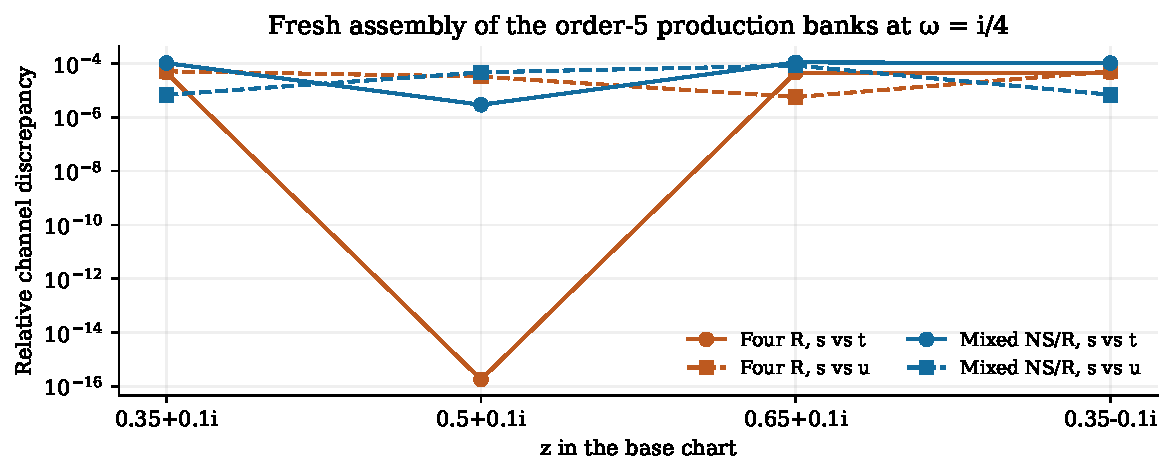
\includegraphics[width=.96\linewidth]{figures/sphere_crossing.pdf}
\caption{Fresh spectral assembly of retained order-five sphere
production banks. Finite block order, momentum quadrature and
self-dual extrapolation remain numerical approximations.
Zero differences are plotted at the \(10^{-16}\) display floor.}
\end{figure}

\subsection{Retained RR torus evidence}
The included normalization report records independent 1369-node
and 676-node spectral integrations at \(\tau=i\), \(z=0.04+0.1i\)
and its modular image. With \eqref{eq:torus-factors} and theta
permutation \((1,4,3,2)\), the maximum relative modular error is
below \(1.10\times10^{-6}\); the quadratures agree within
\(8.95\times10^{-8}\).
The retained 64-node radial/OPE comparisons have maximum discrepancies
\(1.82\times10^{-3}\) bare and \(5.74\times10^{-2}\) raised.
Raised components still require block and spectral refinement.
These larger integrations were not rerun while packaging; the report
and its input hashes are supplied. They do not fix a common
genus-one string-amplitude constant.

\subsection{Type 0B sphere amplitude}
Figure~\ref{fig:amplitude} is regenerated from the retained production
scan without refitting or normalization adjustment. For the tachyon
\(T\) and axion \(A\), the incoming energy is \(\omega=it\) and
the three outgoing energies are \(it/3\). The comparison target is
\begin{equation}
 \mu_F^2{\cal M}_{A\to ATT}=\mu_F^2{\cal M}_{A\to AAA}
 =\frac{it^4(1-2t)}{27},
 \label{eq:matrix}
\end{equation}
with the energy delta function omitted. It is used only after
worldsheet integration, not as an integrand coefficient.
The scan used 32 spectral nodes, physical block orders four and
five, \(b=1.01,1.02\), 60-digit assembly, collision radius 0.18,
and 24-by-48 bulk moduli quadrature. Maximum observed relative
differences are about \(0.02581\%\) mixed and \(0.00247\%\) four R.
These are comparison residuals, not certified absolute errors.
\begin{figure}[htbp]
\centering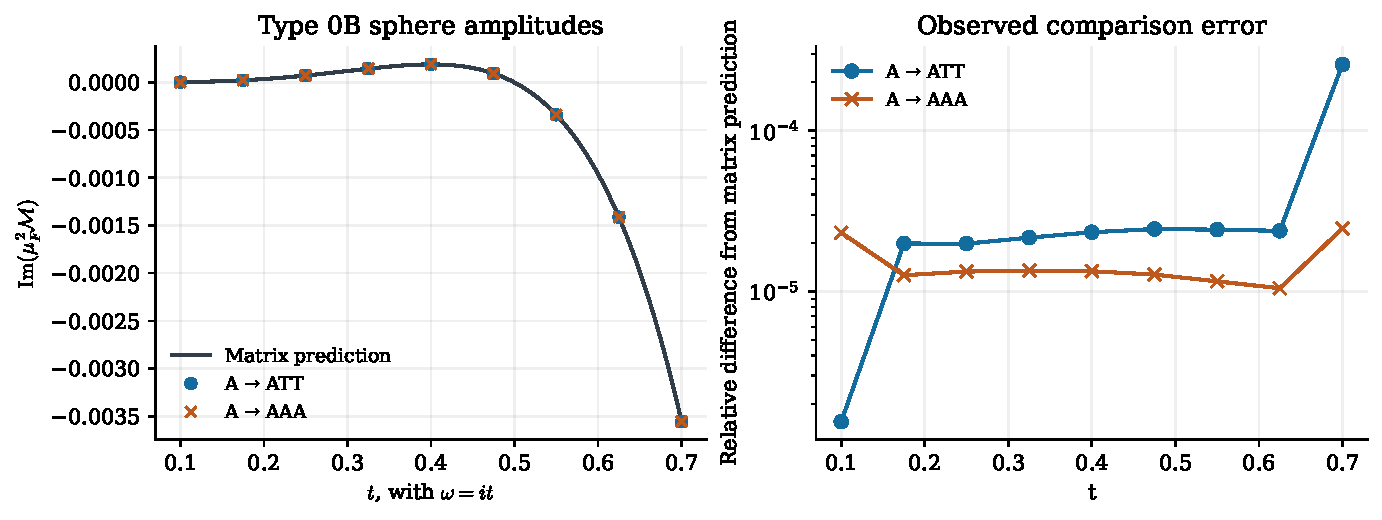
\includegraphics[width=\linewidth]{figures/type0b_sphere_amplitudes.pdf}
\caption{Type 0B genus-zero amplitudes in the local scattering
dictionary. Points are retained worldsheet results; the line is
\eqref{eq:matrix}. Right: measured relative difference.
Data: \code{notes/evidence/sphere\_amplitude\_scan.json}.
No torus amplitude is plotted: the current RR torus still lacks a
fixed absolute string normalization and completed integrated result.}
\label{fig:amplitude}
\end{figure}

\FloatBarrier
\section{Reproduction}
Use Python 3.11 or later from the standalone folder:
\par\noindent
\begin{minipage}{\linewidth}
\begin{verbatim}
python3.11 -m venv .venv
.venv/bin/python -m pip install -r requirements-tested.txt
.venv/bin/python -I -B run.py verify
.venv/bin/python -I -B run.py examples --output-dir results
.venv/bin/python -I -B run.py test --output results/validation.json
.venv/bin/python -I -B run.py cross-check --output results/cross_channel.json
\end{verbatim}
\end{minipage}
\par\medskip\noindent
Edit the JSON examples to change momenta, insertion points or cutoffs.
Complex numbers are \([{\rm real},{\rm imaginary}]\) pairs.
The examples return blocks and fixed-momentum assemblies; the NS
sphere also accepts a finite spectral quadrature. Every output states
its included primary powers, frame factors and measures.
The low example orders are execution checks, not convergence claims.

The included banks cover only the \(\omega=i/4\) crossing check.
The nine-energy amplitude scan is retained evidence for the plot,
not a bundled complete nine-energy integration campaign.
Regenerate both figures with \code{tools/make\_figures.py}.
Ramond zero momentum, confluent poles and branch-cut continuation
need the corresponding limiting prescription.

The practical rules are to retain the local trinion dictionary,
retain its metric and component contractions, apply the RR torus
correlator prefactor only after the descendant sum, and include
each spectral measure and external leg factor once.

\clearpage
\begin{thebibliography}{9}
\bibitem{BRY} B. Balthazar, V. A. Rodriguez and X. Yin,
\emph{The S-Matrix of 2D Type 0B String Theory, Part 1},
\href{https://arxiv.org/abs/2201.05621}{arXiv:2201.05621},
Sections 3.1--3.2 and Appendix A.
\bibitem{Suchanek} P. Suchanek,
\emph{Elliptic recursion for 4-point superconformal blocks and bootstrap
in N=1 SLFT},
\href{https://arxiv.org/abs/1012.2974}{arXiv:1012.2974}.
\bibitem{HJS} L. Hadasz, Z. Jaskolski and P. Suchanek,
\emph{Elliptic recurrence representation of the N=1 superconformal
blocks in the Ramond sector},
\href{https://arxiv.org/abs/0810.1203}{arXiv:0810.1203}.
\bibitem{CCY} M. Cho, S. Collier and X. Yin,
\emph{Recursive Representations of Arbitrary Virasoro Conformal Blocks},
\href{https://arxiv.org/abs/1703.09805}{arXiv:1703.09805}.
\bibitem{source} Local production source and hashed numerical evidence
in this package. Source-specific phases and normalization
qualifications describe these implementations and do not assert
that every convention in the literature has been reconciled.
\end{thebibliography}
\end{document}
